\chapter{疯狂派对}

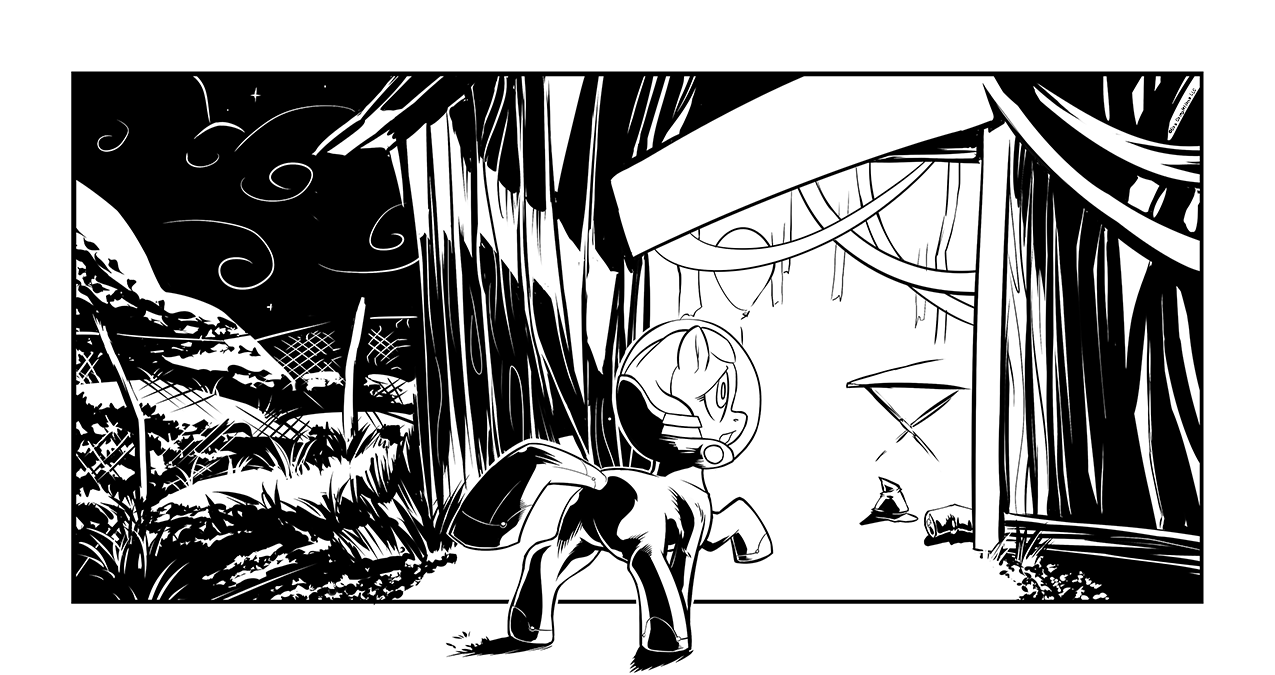
\includegraphics[width=0.9\linewidth]{image02.png}

\begin{intro}
    不需要带上礼物,能来就足够了!
\end{intro}

\daytimeplace{2}{4:00 PM}{赤兔山脉,52号国道北口}{Redtrotters ridges, Big 52 N Branch}

通常来说,穿着一套全封闭式环境适应服一点都不符合小马国时尚审美,但是大家也必须承认它还是能带来很多便利。首先如果你能从一次野火炸弹\footnote{野火炸弹(Balefire Spell):\emph{FoE} 设定之中的几个超聚魔法之一,类似于原子弹}袭击中幸存下来的话,你估计能够享受到渴死在环境服之中的待遇。其次它完全防水,并且基本上隔热,所以你也用不着雨伞或者墨镜。对了还有一点,它是柠檬黄色,所以基本上任何时候你都能被一眼看到。除非……大概……如果……你不小心埋在一大堆柠檬之中的话……那时你肯定不想被任何马看见,对吧?不过,很显然的是在废土上有时候隐匿行踪才是美德。

前提是帕比认识「时尚」这个词的话!

\horizonline

「嗨!我是快乐帕比!」穿着黄色的幼驹对着面前的俩小马微笑着。他们穿着和那天晚上那仨差不多。不过外表少了一些狂野,而且装备更精良。一只独角兽雌驹拿着一把防暴霰弹枪,搜寻着帕比后方是否有什么异常,另一只陆马身边似乎捆着一根大号长矛。要是帕比知道那是什么东西,这两匹雌驹的举动肯定会让她胆怯。

独角兽先开了口:「小鬼,你在赤兔的地盘上干什么?」

「那奇怪的衣服又是什么玩意儿?」陆马接着问。

「我在找我妈妈!」帕比兴奋地回答,伸出蹄子指着路的大概方向。「她在那边!」

俩部族小马相互对视了一眼,然后独角兽又问:「好吧,你妈妈叫什么名字,她是赤兔的?」

「啥是赤兔?」

独角兽的表情开始不耐烦了,不过陆马替她回答了问题。「我们就是赤兔。在52国道上从这里到盐块城都是我们的地盘,所以你想要通过这里,那么你就要通过我们的地盘,所以你妈叫什么?」

「我妈妈叫阴雨·黛丝(Rainy Days)!她超级酷而且总是给我唱歌,还会做很多好吃的!她是最棒的小马!等长大了我也要变成她那样!」

「好了,好了,我知道了。」独角兽不爽地打断她。「抱歉小鬼,但是我不认得什么阴雨,她肯定不是赤兔,你是独自一马吗?谁送你到这儿来的?」

「我有声音先生陪着我!」

「声音先生?」独角兽再次警惕地巡视着道路。

「是啊!他住在我的太空服里,有时候我们一起唱歌,但有时他的脾气也很暴躁,但没关系,因为他会帮我找到妈妈!」

「好吧。」雌驹松懈了警惕。「这样,我很抱歉,但如果你和你的隐形朋友想要通过这里,就得交路费。」

「啊……好滴?我有……」帕比开始在她衣服上的口袋上翻找起来,一路上她收集了不少好东西,大多是一些坏掉的玩具,还有她觉得有趣的东西。或许她可以分一些给这些小马。毕竟我们要彼此体谅,彼此分享\footnote{彼此分享,彼此体谅(You gotta care, you gotta share):这是S01E21中萍琪派的歌词},不是么?

「那么这个怎么样?」

不能用牙齿拿东西是一个很大的问题。她不得不改用她的蹄子,但笨重的橡胶靴使这项任务变得更加艰巨,而且她必须以十分尴尬的角度弯曲她的腿以便伸入她的鞍包。

「等等,我马上就能……呃……」

「{\mt 提示:该防护衣提供简单的操作魔法,可以通过HUD菜单来访问您的物品栏选择物品。}」

「啥?」

陆马看着帕比嘟哝着从她的鞍包中捣鼓出各种无用的垃圾。这个小家伙肯定没有什么值钱的东西。拿长矛的小马看着她的朋友使了个眼色。她若有所思地叹了口气,在对残酷的命运之神进行了短暂地内心祈祷之后,将长矛插入了小马驹的脖子上。快乐帕比忙着听她那衣服发出的各种抱怨。她像一堆砖头一样倒在地上,陆马将她放倒后,默默地咒骂着废土。

「你这是帮了她。如果没有她母亲,她连一天都活不下去,而且我们也不能把她带进来。这样总比让她被蝎尾狮吃掉好,或者比那更惨。你知道这里的小马驹会发生什么。」独角兽叹了个口气。

陆马注意到了独角兽的复杂表情,她补充道:「是啊,可怜的瑞吉……」

长毛马从尸体上拔出武器。当她退后一步时,粉红色的烟雾开始从衣服上的洞中逸出。雌驹注视着这个现象,疑惑不解。「嘿,瘦子,那是什么?」

独角兽用蹄子抓了抓头,「你肯定戳坏了防护服的某个魔法晶片……这东西可能有毒,我们站远点。」

「我们总不能把尸体留在这儿吧,感觉不太好。」陆马犹豫着,但还是躲开了粉烟。

「在你弄出那么多烟火之后,我可不打算靠近她!红蟑螂会解决她的。我们走吧,继续巡逻。」

俩小马最后看了倒在地上的小幼驹一眼,小跑着走开了,离开大路,然后爬过一个低矮的山脊,消失了。时间从路中间黄色幼驹的身体中流过。一阵冷风刮来,在光秃秃的树上沙沙作响。尽管有风,围绕着她的粉红色的云烟似乎也没有消散。

\horizonline

\daytimeplace{2}{4:30 PM}{赤兔山脉,52号国道北口}{Redtrotters ridges, Big 52 N Branch}

在一阵咯咯声之中,防护服发出的声音表示这个故事还能继续讲下去。

「{\mt 初始化系统。检查版本。警告,版本号匹配错误。启用安全模式。版本 0.2。检查装备状态。所有系统上线。检查到大型破损。激活修复魔法。恢复上次会话。读取目标001的个性化信息:快乐帕比,目标已死亡,体征稳定,检测完毕。}」

帕比的双眸在头盔里面眨了眨,就好像她刚刚睡醒了一场长觉。小幼驹打着哈欠,一滴粉色的口水从嘴角落在玻璃面罩上,但是立刻就被玻璃吸收了。

「唔唔……再睡五分钟,妈妈……」幼驹打了个滚,依然被那慢慢消散的粉云包围着。

「{\mt 破损修复,目标已经与危险环境隔离。}」

小雌驹睡眼惺忪地看着四周,先是皱着眉头,然后她似乎想起来什么。「哦,对了,妈妈不在,我刚刚怎么睡着了?」帕比想抓抓头但是蹄子被头盔挡住了。所以她眉头皱得更深了,非常不开心地耸了耸肩,并且若有所思地抱着头盔。

「{\mt 读取临时记忆,提示:失去信号之前最后一个行动,商谈买路钱。}」

「商谈啥?」

「{\mt 与赤兔商谈经过领土的通行费用。}」

% NOTE: 漏译

又来了。「鱼翅……啥?」

「{\mt 和漂漂小马聊天。}」

终于,小幼驹听懂了!「哦,对哦,漂漂小马!我想起来了!啊……他们哪去了?」

「{\mt 赤兔位置未知。将寻找该目标增加到任务清单中。}」

帕比一脸为难的抬起眉毛。「你们还要列个清单?从什么时候开始?」

「{\mt 清单在23小时之前创建。清单上项目:4项}」

「哇哦,我们还真有不少事1、2……呃……4是个好大的数啊,是吧?清单上有什么?」

「{\mt 主要目标:到达MoM。次要目标:解决防护服问题。次要目标:确认马尾伯爵或者至少回避他。次要目标:寻找赤兔。}」

在听完这个清单之后,一脸沉思表情的黄色幼驹戳着自己的头盔。「动动脑子,动动脑子……马芬!不……等等……不是那个……」几分钟之后,幼驹点了点头,双眸闪着光,「哦哦哦!放点音乐……啊……那个话挺多的小马台。」帕比一边听着广播,一边跟着箭头继续她的旅程。

52国道附近的荒地全都是小山和石头,这个地形的视野非常糟糕。这通常会带来很多不便,不过帕比一点都不在乎。

「嘿,声音先生,你刚才说什么关于口袋里面拿东西的事情?」

「{\mt 肯定。这个衣服装备了基础的操作魔法。}」

「呃……怎么用?」

「{\mt 读取说明。选择为幼驹和小呆准备的简单版。说出你要的物品名字,符合描述的物品会悬浮到你面前。}」

「啊……马芬!」一盒200多年前的马芬浮到了帕比面前,她咯咯的笑着,这东西在天上飘着的样子看起来傻乎乎的。

「嘿嘿,好好玩!黎明沙士!」一瓶黎明沙士代替了马芬。「玩具车!」这次一个看起来坏得很厉害的玩具车浮在了幼驹面前。「嘿嘿!我们应该多找点东西,我喜欢这个猜谜游戏!」

「{\mt 否定。这不是猜谜游戏,这是物品管理系统。}」

帕比拿起一块石头放进口袋里面。「石头!」石头立刻浮在了她面前。「耶!真灵!」当石头放回去的时候,石头的名字变成了「命运之石(The Rock Of Destiny)」,但是帕比基本不识字,所以她也没注意。

幼驹一边继续顺着路走着。一边不停地要着物品栏中的东西,其实并没有多少,总共她也只有四件东西,但是她有个大计划。

「哦,我们需要更多音乐!」

\begin{music}
千里之外那指路之星闪耀天穹

\begin{englishlyric}
    I can see that lone star from a thousand miles away
\end{englishlyric}

\medskip

指引迷失的我踏上家乡的归途。

\begin{englishlyric}
    Calling me back home, though I ventured far astray.
\end{englishlyric}

\medskip

当我向着那个灯塔勇往直前,

\begin{englishlyric}
    When I see that beacon shining for me all alone,
\end{englishlyric}

\medskip

它带我飞翔带我回到家乡回到小马国!

\begin{englishlyric}
    It calls me back to `Questria and my home!
\end{englishlyric}
\end{music}

\horizonline

\daytimeplace{2}{7:00 PM}{赤兔山脉,52号国道北口}{Redtrotters ridges, Big 52 N Branch}

这里的居民点看起来比棚户区稍微强那么一点点,至少没有拿臭水沟当护城河什么的。它的城墙看起来更像是一辆撞毁在民宅上的旧汽车,而不是什么防御设施。

帕比完全没有在意这些,一路蹦跶进城里,摇头晃脑地唱着电台里面的歌曲,一直到她面前地面上暴起一团尘土。

「嘿!你,我说了,给老子站住!」

帕比回头看着「城墙」,大概50多米远的地方有个小马举着一个大枪对着她。于是幼驹坐下来挥着蹄子微笑着。「嗨!我是快乐帕比!」

在那堆破烂后面举着大号来复枪的小马显然没有被她的热情感染到,板着脸说:「好吧,拿下那个大金鱼缸,我要看看你的脸!」

「呃……我真的很想这么做,但是我卡在里面了!」帕比想了想说:「实际上,这件事还在我的清单上!」

「好吧,你行……呆在那里把蹄子和武器都放在我能看得见的地方!」

「我不觉得我有什么武器……我有一块石头,算么?我可以丢它!」她蹦跶着说。

卫兵无奈的以蹄覆面,「喂,大号你去搜她身,你,黄色的小个子,给我乖乖站好!」

「好的,好滴,好得!」帕比笑着,不过她的回答显然让那路障后面的小马不满意。

「回答『是』就行了,只要别耍花招,要想大家都没事,就呆着别乱动,让大号做好他的活。」

棕色的大个子雄性独角兽走到帕比身边,看着幼驹在头盔后面的那张笑脸,她双眸之中的光亮现在小得几乎看不到,完全被头盔上各种HUD的光掩盖了。

「我擦,你穿的这身防辐射服保养得可真好……从没见过这样的……」

「当然!它超黄超聪明的,还可以变戏法!你看!嗯……马芬!」刚刚的那个马芬盒子立刻飘到帕比面前。

「哇哦,内置物品管理系统和次级操作魔法,这东西绝对贵得要死,你从哪儿弄到的?」

「中心城的一个漂漂小马给我的!」

「这么说……你来自中心城?」大号听起来不太相信她说的。

幼驹自豪的点了点头。「没错!」

「就是52号国道能看到的那座大山上的城堡么?」

「就是那儿!」帕比笑着回答。

「哦,怪不得你穿着全封闭防辐射服……好吧,我们别闲扯了……给我看你的通行证。」

帕比茫然的看着棕色独角兽,「我的啥?」

「你没通行证?你来的路上没碰到巡逻么?」

「我看到俩小马,一个像我一样的陆马,还有一个是……犄角……单角……哦哦……独角兽!他们超和善超漂漂!」

「没错,没错……好瘦子和冰苏打」大号打断了她后面的话。「他们没和你提什么买路钱之类的?」

「呃……不太记得了。我们聊了一会,然后我有点犯困他们就丢下我走了。」

「随便从她身上拿点什么然后给她个通行证!」

「呃……好吧……」

那小马搜了搜帕比身上,但是除了石头和衣服没啥东西,他甚至想解开那外套,但是不管他怎么弄看起来都没什么用。「好吧,很抱歉小鬼,我也是迫不得已……」他们给了帕比一个中间染了红色的破锡罐。「给你,给幼驹的特别折扣。」

「我会告诉我妈妈你们对我很好,谢谢你们漂漂小马!」

「就这样吧……说起来,一个幼驹穿着防辐射服自己在52号国道溜达?这里可不是什么好地方……」

「我去找妈妈!」帕比看了看附近似乎想要找个标志物,然后指着东南方说:「就是那边,好了我走了拜拜!」幼驹不等他们回答就走掉了。

「但是在哪个方向的就只有嘉年华……啊等一下小鬼!那里很危险,别去那里!」大号举起蹄子,但是转念一想,她和他非亲非故,在废土这种地方多一事不如少一事。

黄色的小雌驹继续顺着小路往前走,她看到那条弯弯曲曲的小路上有一些马为的痕迹,不知道谁在路里埋了很多削尖木棍。帕比在小路上闻了闻,然后就再没管它,在石头上爬上爬下,跳来跳去的游戏对于一个这么大的小幼驹来说是超有趣的。随着夜色慢慢变深,幼驹也渐渐走进废土深处。

\horizonline

\daytimeplace{2}{10:30 PM}{嘉年华,废土}{The Carnival, Wasteland}

一个巨大的谷仓坐落在小小山谷之中,从上面斑驳褪色的痕迹可以看得出它曾经漆成粉色。它被环绕山脊的栅栏包围着,栅栏上每隔一段就有一个自动炮台。这幢建筑和栅栏还有炮台都已经破旧不堪,但是那些炮台依然颤颤巍巍地来回转动着保卫这里。

「{\mt 警告,侦测到自动防御炮台,敌对模式。威胁等级:中等。}」

敌对这个单词让帕比立刻警觉起来,她站定了看了看四周,「那伯爵又来了?在在哪?那马还真纠缠不休,呃,我觉得还是小心驶得万年船。」小小马连忙躲在一个石头后面,警惕地看着那个马尾伯爵先生是不是追来了。「关了音乐,声音先生,我们在躲猫猫呢!」她屏住呼吸竖起耳朵听着周围。

「{\mt 开始和防御系统建立通讯连接。交换协议。申请进入。申请成功。路障已清除,请继续前进。}」

「我说安静!附近肯定有小马……或许是那伯爵,我们应该超级小心!」帕比从掩体后面探出头来,回头看着附近以免有什么可怕的东西就在她身后,然后她慢慢走过栅栏,炮塔马上指向她的方向,但是它们在罗盘上的红点从红色变成了粉色,炮塔又回到了它们通常的防御方向。

「嘿,声音先生……我叫你别放音乐了……」

「{\mt 肯定。无线电已静默。}」

「那么为啥我还能听见音乐?」

「{\mt 声源检测。音乐来自MoM建筑物。}」

「里面?妈妈在谷仓里面?还有音乐和其它东西?妈妈在开派对?耶!」帕比立刻停止了躲藏,四蹄并用从山坡上直奔谷仓大门,最后幼驹猛地踢开大门跳了进去。

「惊喜!」

谷仓里面的空间非常大,而且很开阔,还有两个阁台,一个在门上方,另一个在对面。地面整理得很平,并且铺了一层稻草,墙壁上挂满了破旧的彩带和花环。屋顶上吊着几个看起来很惨的糖罐,还有一大堆灯泡、没气的气球还有其它破烂不堪的旧东西。几盏勉强能发出光亮的旧挂灯无精打采地照亮着这里,唯一看起来能正常工作的就是那个凑合能发出点儿声音的破旧喇叭。

在屋子的正中间有一个派对长桌,桌边已经有一些客人了——一袋面粉,一堆石头,一个装了不知道已经烂掉的什么东西的锈桶,它们都带着一个派对帽\footnote{此处可参考正剧《独马派对》}。哦,座位上还有很多骷髅,至少一打了无生机的小马坐在桌子边,头上带着派对帽,空旷的眼洞看着面前空空如也的盘子,甚至有几个看起来像是干掉的木乃伊而不是骷髅。实际上,其中之一看起来像个饿到皮包骨的小马,而远处的角落堆着一大堆白骨。

「{\mt 警告,侦测到轻微辐射。警告,空气中检测到毒气。分析中,毒气成分:一氧化二氮\footnote{一氧化二氮:无色有甜味气体,又称笑气}。威胁等级:微不足道。}」

「哦,看呐,新客人!」一个看起来像是派对主持的影子从座位上站了起来。那是一只金属的小马,发出旧唱片一样的吱吱声。在昏暗的灯光下,她看起来就像是一只长着粉色鬃毛的粉色小马,但是靠近之后,帕比发现到她是靠轮子移动的,就好像她蹄子下面穿了电动滑冰鞋一样!「看看你的样子!我想你是来这里参加化妆舞会的,不过我很抱歉通知你舞会已经取消了!但是你可以继续穿着你的外套!因为超酷!」另外一件奇怪的事情是,一般小马说话的时候嘴巴会动,但是这个小马印在脸上的微笑却完全不会动,取而代之的是她在说话的时候眼睛却会诡异地闪闪发光。

「呃……你是个……机器马?」帕比迟疑着问,因为她想起来妈妈告诉她如果其他小马看起来很奇怪不要随便当众说出来。

「那是,当然!你真是个聪明的小马!我是娱乐用机器萍琪 MK II 原型 03 号,这是我的生日派对!想要加入么!我可以给你腾出位置,你知道的,有些客人有些不开心,坐在那里不说话。」

「呃……我是快乐帕比……我……呃……我找我妈妈……她应该在这边……大概?」

「太棒了!等她来之后她可以一起加入我们!现在坐下来,你想要吃点蛋糕么?」

帕比没有参加派对的兴致,她应该能在这里找到自己的妈妈,而不是这个破烂生日派对……或许和这个机器马一起玩一会之后她可以帮她。所以幼驹坐在位置上之后看着其他客人。

诡异这个词已经不能形容现在帕比的情况了。那些骷髅正在看着她,所有那些死掉的东西还打扮得像派对来宾一样,尤其是那俩超级瘦的木乃伊……

等等!一个木乃伊居然转过头来了?「求你……哈哈哈……别让我……哈哈哈……笑了……」她还说话了!

这个小木乃伊是一只有着浅黄色毛皮和橘色鬃毛的独角兽,她看起来病得很厉害,幼驹笑个不停但是看起来却一点都不开心,似乎她只是止不住要笑。她眼睛很空洞,而且鼻血流个不停,鲜红的鼻血流得她浑身都是。「求……呵呵……让我回家……」她喃喃地说着这些话,似乎她已经说了上千次,可她仍然在不停地说着,好像说够了次数之后就能从这个噩梦醒来一样。

帕比感觉背后一阵恶寒,好像后背滑过一块冰块似的。这地方不对劲,她想走。但是妈妈在这里,她可能……可能是……那堆……骷髅的……其中之一。

惊恐万状的帕比几乎不能自已。这简直就是那个原本超级和善的机器马觉得烦了,于是就开始伤害小马的故事翻版!已经有太多的小马死在这个毛骨悚然的嘉年华派对上,而马上还会有更多牺牲品!而且她妈妈可能还在邀请名单上,如果她……不对如果她已经……等等!那机器马似乎说了什么她不在这里的话?但是那个机器马可能在说谎。她会说谎么?谁还管这个!这个粉色的东西绝对是个大坏蛋,帕比不想再和她玩了!

那一瞬间,帕比的视线和那个坐在桌边咯咯笑的小幼驹相交,那小马也想她自己的母亲,这里是个坏地方!「快跑,快回家!」帕比看着她,一直到小独角兽离开座位。机器萍琪走过去打算拦住她,但是帕比正要找它算账。

「我妈妈在哪里?」她从座位站起来问。

「等派对结束我们可以一起去找你妈妈,好吗?要不要来点儿黎明沙士呀?」

小独角兽趁机一步一捱地挪向门口。

「抱歉,派对还没结束,你不能走!」

「我妈妈在哪里?」帕比走向那个粉色的马形机械,吸引她的注意。

「好了,好了,乖乖的,别坏了派对兴致。你想玩钉马尾游戏么?」

粉色的火花在帕比双眸中燃烧。「我妈妈在哪里?你把她怎么了?」

「错误。物件妈妈未找到。拜托,别生气。我觉得你妈妈很快就会来接你的!」小独角兽回头看了一眼,靠着大门勉强让自己站好,她颤颤巍巍地走着就像一个乌龟一样。机器萍琪滚着轮子走向她。「站住别动!长辈没允许,不准离开!」

「不要忽视我!她应该在这里的!讨厌的机器马!我不会让你再伤害别的小马,不会让你伤害我妈妈!」帕比低头弓起身子,「石头!」她低声咆哮着。

「请不要说脏字,开始镇压行动,目标免疫毒气,需要使用物理力量,建议使……」

咣当!

「我!」帕比双眸明亮地闪烁着,头盔上反射着粉色的火光,黄色的幼驹直接跳在机器马脸上,不停地用「命运之石」用力砸她。

「妈妈!」帕比咆哮着用双蹄抓着机器马的脖子,拿出自己吃奶的力气和它头碰头,力气大到头盔上都撞出了蜘蛛网一般的裂痕,同时也撞坏了机器萍琪的脸部面板,露出了后面的电路和机械组件。

「在!」帕比一只蹄子继续抓着机器马的脖子,另一只蹄子不停地砸着漏出来的电线,每一下都会让机器马脸上飞出一些被打烂的电路和零件,直到她砸到一个魔法晶片。紧接着机器马就像身体里塞满了粉色和黄色烟花一般炸开了,把帕比炸飞到房间另一头。

「哪里?」被炸飞的帕比一屁股坐在了一座自动炮台上,这东西在她打烂了那机器萍琪之后就冒了出来,电子的爆裂声就像是在悲鸣,那炮台顿时爆成了一团火花,剩下的炮塔则锁定了帕比射出无数五颜六色的激光弹幕,不过那些光线完全无法射穿帕比的防护服。

「别闹了!告诉我,我妈妈去哪了?」帕比径直冲向其中一个炮台,用力撞向它,撞得它歪向一边,而那炮塔还在疯狂的射击着,所有弹幕都打在了天花板上,对于破旧的木质建筑而言,激光的破坏力可比对一件涂有反射材料的防护服有效得多,帕比转身一蹄子把它从底座上踢飞了下来。虽然那机器闭嘴了,但是天花板同时也裂开了。

「妈妈!妈妈你去哪了?妈……妈!」完全不管正倒塌在她周围的谷仓,幼驹疯狂地跑向角落的骨头堆。「声音先生,你看见我妈妈了么?她在哪里?」

「{\mt 错误,地点已到达,斗志部分部已经找到。}」

「你又说什么乱七八糟的?我要妈妈!你说她在这里!」

随着最后一声低沉的隆隆声,历史久远的谷仓终于整个垮下来砸在了帕比的小脑袋上。

黎明的第一道光芒照亮了废土之上永远不散去的云层,一个娇小憔悴的独角兽小雌驹从前MoM建筑倒塌的烟尘之中爬出来。炮台静静地躺在哪里,因为已经失去了动力源,就连音乐声也消失了,持续了200年之久的挽歌终于结束。只有几丝火星在废墟之下闷烧着,吞噬着那些残存的朽木。

\horizonline

\daytimeplace{3}{9:15 AM}{嘉年华,废土}{The Carnival, Wasteland}

即使到现在,这个被诅咒的地方依然没有找回安宁。

「我没有让你找这个可怕派对地点,我让你找我妈妈!」废墟下面闷声说。

「{\mt 否定,你说了……}」外套播放了帕比之前说话的录音。「声音先生……妈妈在哪儿?」

「我就是这么说的!」

「{\mt 肯定。斗志部最近的可用分部已经定位并且标示在地图纸上,并且在几小时前已经被设定为主要任务目标。现在它已被摧毁。}」

「不用你说,它爆炸了两次。」

「{\mt 否定。它不可能爆炸两次。主要损害已修复,系统运转正常等待下一步指令。}」

帕比静了静,整理了一下思路。对声音先生凶也没有用,主要是因为没什么东西可以揍,所以她应该聪明点,她是个聪明孩子,对吧!反正那个机器萍琪是这么说的!

「好的好滴好得……覆水难收……或者说,坏谷仓没法修……既然你说妈妈不在这里,那么然后去哪里?」

「{\mt 警告,尽管已经解释完毕,但现在依然有一个重大误……}」

「喂,闭嘴啦!下一个妈妈可能会在的地方是哪里?」声音先生该不会是因为一直干活不能玩,所以闹脾气了吧……笨衣服……

声音沉默了一会,如果他有更复杂的智能的话,他可能会说些别的,或者至少觉得沮丧,但是这个程序就只是为了服从命令,他只能做到这一点。

「{\mt 下一个MoM地点定为主要目标,位置已经显示在罗盘上。}」

在帕比终于把自己从废墟里面挖出来的时候,一个新的粉色箭头出现在罗盘之上。幼驹跳下碎石堆,抖了抖身上的尘土然后说。

「看到了吧,如果你合作的话什么事都这么简单。」

「{\mt 肯定,合作是魔法。}」

一个金属的笑声打断了这场对话让帕比抬起了头,她看到几天前见过的那个嗡嗡响的机器精灵。

「哦,是你啊提问者,嗨!」幼驹微笑着。

「是守望者……不管怎么说这都太无厘头了吧?」

「什么?你说这个派对?你信我的,你啥也没错过,这是最烂的派对,没有之一,所有小马都无聊到死,呃,真的死掉了。」

「那么,找到你妈妈了么?」

「完全没有。」帕比微微皱了皱眉头,然后又笑了起来。「但是我们还有很多地方要看看,所以没问题!她肯定在哪里,对吧?」

「呃……大概……吧?」机器顿了好长一会儿,「顺便,我可以问问你打算去哪么?」

「那边!」小雌驹用蹄子指着,然后补充道,「这次我觉得会走运!」

「所以,你打算检查下一个『MoM』地点?」

「当然!」

机器又一次顿了很久,「你还觉得下次会走运?」

「没错!」

「好吧,的确是,反正已经……很好,帕比,我该走了,祝你旅途愉快。」

「当然,提问者先生!祝你一路顺风!」机器精灵转头飘走了,还大声广播着贪食精灵进行曲。

「哦,对了!声音先生,来点音乐吧!」

\begin{music}
我不想把整个小马国点燃,

\begin{englishlyric}
    I don't want to set Equestria on fire,
\end{englishlyric}

\medskip

我只想点燃你心中的激情!

\begin{englishlyric}
    I just want to start a flame in your heart!
\end{englishlyric}
\end{music}

\horizonline

\daytimeplace{3}{2:00 PM}{赤兔平原,52号国道北口}{Redtrotters Flats, Big 52 N Branch}

帕比回到了52国道。把那些山丘抛在脑后之后,眼前出现的是一望无际的大平原。远处大城市摩天大楼的剪影面前,点缀着近处一些旧农舍的残骸。在路边有很多旧的马车,有一些是轻巧的小车,有一些是载货的大车。它们都面临着同样的命运——独自在路上锈烂。

「嘿!说你呢,等等!」帕比转向叫她的声音来的方向。

黄色的小雌驹看到过来的是昨天那俩母马,她微笑着挥舞着蹄子,她们其中之一在30米开外停了下来,并举起一把突击步枪,另一个慢慢靠近,并且谨慎地举着动力长矛。

「好的,我的神奇小丫头,乖乖站好大家都不会受伤。」

「呃……我们在玩游戏么?」

独角兽继续用枪瞄准着帕比,另一个小马回答道。

「没错,差不多,想要玩么?」

「好棒!我可以先来么?可以么?可以么?可以么?」帕比已经开始和她这个年纪孩子一样兴奋的上蹿下跳了。

「当然,我们玩我问你答游戏,你如果答不上来你就输了!懂么?」

「耶!猜谜游戏!我超喜欢猜谜游戏!问我,问我什么都行!」

「好,第一问:为什么你嗓子眼被动力长矛戳过之后还活着?」

「啥和啥?」这个问题太难了,帕比完全不知道什么是动力长矛,听起来似乎是吞下什么东西并且不被噎到的意思。「呃……可以略过这个问题么?」

俩母马交换了一个眼神。「或许,这家伙只是个笨小孩?」陆马提议道,独角兽叹了口气,「好吧,我们问问别的事情。」

「好吧,小鬼,那么……为什么你去嘉年华?」

「你是说那个旧农场?好吧,这个傻蛋声音先生告诉我妈妈在那里,你猜结果怎么回事?她没在那里,而且那里还有个全世界最无聊的派对,那个发疯的粉色机器马还想伤害我妈妈,我很生气,但是机器马爆炸了,然后有个怪东西开始往我身上照讨厌的光线,剩下的我记不太清了,只记得整个农舍都砸我头上了,最近真是被房子砸了好几次……」帕比想了一会,又补充道。「我希望那个瘦瘦的孩子能安全回家。」

「瑞吉还活着,所以我朋友还没开枪打你。」陆马深吸了一口气。「所以你复活了以后走了这么远跑到嘉年华,然后把那个天杀的地方毁了,并且救了瘦子的妹妹,这一切只是个意外?」

「我……我不记得我做了那些事情,不过既然你这么说……」

「然后你一直只是在找你妈妈?」雌驹抬起眉毛,疑惑地问道。

「是的,你知道她在哪?」

「没错,她就只是个笨小孩。」陆马无奈地以蹄覆面,而独角兽在她身后大笑着。

笑过之后,独角兽表情变得严肃起来。「不管怎么说她救了我血亲,我欠她的。」

「那么你想怎么办,瘦子。」陆马问。

「我不知道。」瘦子放下枪口靠近那个冲她微笑的快乐帕比。那天真无邪的小小微笑融化了这个铁血女独角兽的铁石心肠,她将一只蹄子放在帕比头盔上。

「我不知道你是好是坏,不过我欠你一次……所以,谢谢。」瘦子递给她一个金属片,上面刻着一颗吃了一半的白色苹果,「拿着这个,这是通行证,如果你去盐块城,把这个给卫兵看他就会让你进去,懂吗?」

帕比睁大眼睛看着她收到的馈赠。「哇哦,谢谢!礼物,我超喜欢礼物!漂亮的大姐姐非常感谢你!」

独角兽继续说:「你终结了我们一族的噩梦,还救回了我唯一挚爱的血亲,我希望你能找到你所寻找之物,小小幽灵。」

「哦哦哦,你也有这么可爱的时候?」陆马低声揶揄着。

「给我闭嘴,赶紧走,苏打,我们还在巡逻呢!」

「嘿,你哭了,瘦子?」

「你闭嘴好么,绝对不准和其他马提起这件事!」

「好吧,说起来,现在我对之前杀过她有些愧疚了。」

两只小马向着粉色箭头相反的方向走开了,帕比挥着蹄子目送他们消失在山脊之后。

「我喜欢漂漂小马,她们真漂亮!」帕比笑着,然后出发走向大城市。

「嘿,声音先生,我可以问你一些事情么?」

「{\mt 肯定,请陈述您的请求。}」

「等我们找到我妈妈之后,你会离开么?我是说……我不想让你走。」

「{\mt 否定,在幼角药剂的影响下,该装备已经永久与您融合。}」

「呃……这就是说,我们能永远在一起?我找到妈妈以后还能和你在一起?」

「{\mt 肯定。}」

帕比微笑着,和往常一样只听她想要听的事情。

「好的声音先生,你已经知道我们现在该干啥了吧。」

「{\mt 肯定,基于数据分析,对您的日常需求预测现在有95\%的准确率。}」

广播开始播放声音,帕比一边唱一边走下去。

\begin{music}
你和我,在一起,

\begin{englishlyric}
    You and me together will be,
\end{englishlyric}

\medskip

在一起,在一起,

\begin{englishlyric}
    Forever you'll see,
\end{englishlyric}

\medskip

我们是,好姊妹,

% NOTE: 兄弟 -> 姊妹

\begin{englishlyric}
    We two can be good company,
\end{englishlyric}

\medskip

好姊妹,好姊妹

\begin{englishlyric}
    You and me
\end{englishlyric}

\medskip

你和我,好姊妹……

\begin{englishlyric}
    Yes together we two\dots
\end{englishlyric}
\end{music}

\clearpage

~\vfill

\begin{note}
升级。我想我们早讨论过这个问题了吧。

否定。升级是辐射小马国同人的既定内容。

好吧好吧,真烦,我可以理解帕比的心情了,那么这样。

增加任务专长:升级是命令——现在你可以正常升级了,耶!
\end{note}





